\documentclass{beamer}
\usepackage{xcolor}
%\usepackage{fontspec}
%\setmainfont{Georgia}
%\usepackage[T1]{fontenc}
%\usepackage{winfonts}
\usepackage[backend=bibtex]{biblatex}
\renewcommand{\sfdefault}{georgia}
\graphicspath{{./Images/}}

\bibliography{report}

%%%%%%%%%%%%%%
% Soton colourscheme

%primary palette:           RED    GREEN  BLUE
\definecolor{sotonblu}{rgb}{.00392 .26275 .34902} % soton blue
\definecolor{sotongrn}{rgb}{.00000 .44706 .45882} % soton green
\definecolor{sotoncya}{rgb}{.03922 .58824 .66275} % soton cyan
\definecolor{sotongry}{rgb}{.19608 .23922 .26275} % soton grey
\definecolor{sotonbei}{rgb}{.59216 .61961 .27059} % soton beige
\definecolor{sotonmet}{rgb}{.73333 .73333 .73333} % soton metal

%some secondary colors:
\definecolor{sotonyel}{rgb}{.99999 .70196 .00000} % soton yellow
\definecolor{sotonora}{rgb}{.99608 .24314 .07843} % soton orange
\definecolor{sotonred}{rgb}{.94118 .05882 .17255} % soton red
\definecolor{sotonrus}{rgb}{.67059 .07059 .06275} % soton russet
\definecolor{sotonbrn}{rgb}{.54118 .25490 .16863} % soton brown
\definecolor{sotonpnk}{rgb}{.88627 .41176 .62353} % soton pink
\definecolor{sotonppl}{rgb}{.32549 .12157 .26667} % soton purple


\setbeamertemplate{background canvas}[vertical shading][top=sotonblu,bottom=sotoncya]
\setbeamercolor{background canvas}{bg=}
\setbeamercolor{button border}{bg=sotonblu, fg=sotonblu}
\setbeamercolor{button}{bg=sotonblu, fg=DarkRed}

\setbeamercolor{frametitle}{fg=sotonyel}
\setbeamercolor{alerted text}{fg=sotonyel}
\setbeamercolor{normal text}{fg=white}
\setbeamercolor{titlelike}{fg=sotonyel}
\setbeamercolor{author}{fg=white}
\setbeamercolor{date}{fg=white}
\setbeamercolor{item}{fg=white}

%%%%%%%%%%%%%%%%%%%%

\title{CDT for Next Generational Computational Modelling (NGCM):\\ High Temperature Nano-Magnetic Materials}
\author{Jonathon Waters\inst{1}}
\institute{
	\inst{1}
	Engineering and the Environment,\\
	University of Southampton,\\
	UK\\
	
	Contact: J.M.Waters@soton.ac.uk
}
\date{}

\begin{document}
\frame{\titlepage 

\includegraphics[height=1cm]{sponsor-wo.eps}\hfill
\includegraphics[height=1cm]{uos_grey_large.png}}

\setbeamertemplate{headline}{
	\vskip25pt % horizontal line
	\vskip-21pt\hspace{2pt}\hfill
\includegraphics[height=7mm]{sponsor-wo.eps}\hspace{3.5mm}
\includegraphics[height=7mm]{uos_grey_large.png}\hspace{3.5mm} % logo on the right
}

\setbeamertemplate{footline}{
	\vskip-8pt % horizontal line
	\hspace{12cm} \insertframenumber/\inserttotalframenumber
	\vskip4pt
}

\begin{frame}
	\frametitle{Speaker Background}
	\begin{columns}
		\column{7cm}
		\begin{itemize}
			\item{2010 - 2014: MPhys(Hons) Physics with Theoretical Physics at the University of Manchester.\newline}
			\item{Summer 2013: Worked at the Deutsches Elektronen-Synchrotron (DESY) as a member of the ATLAS project.\newline}
			\item{2014 - Present: Member of CDT in NGCM}
		\end{itemize}
		\column{5cm}
		\begin{center}
			
\includegraphics[width=3.5cm]{hardhat.jpeg} \vspace{2mm}
			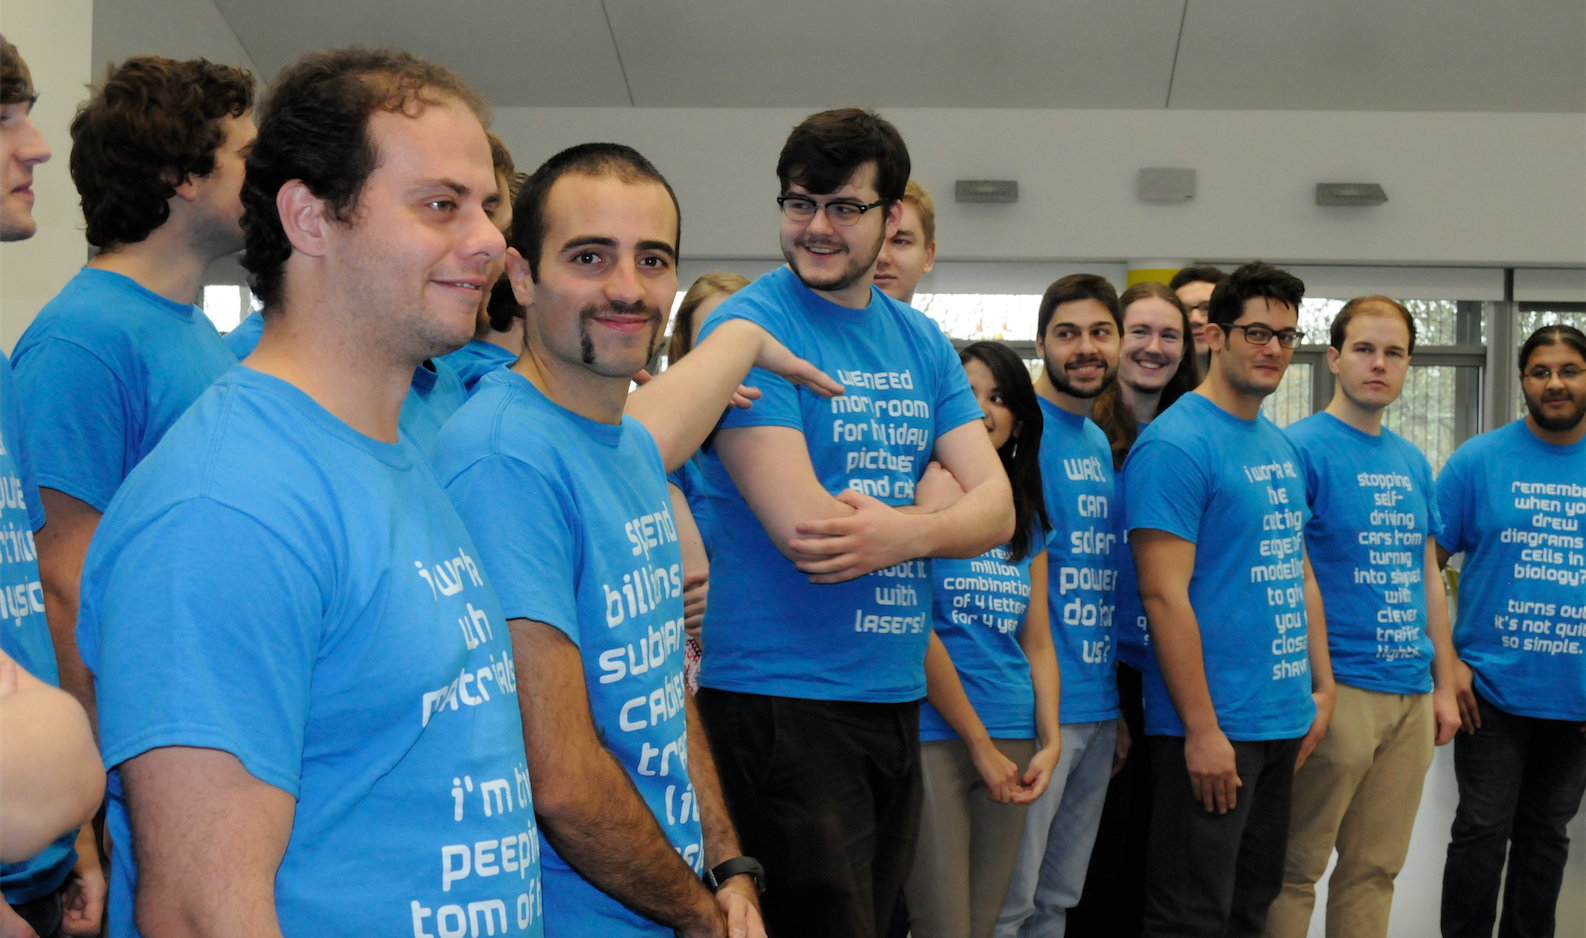
\includegraphics[width=5cm]{ngcm2.png}
		\end{center}
	\end{columns}
\end{frame}

\begin{frame}
	\frametitle{My Research}
	The primary goal of my research is to develop a \textbf{multiscale} model of \textbf{granular} magnetic materials at \textbf{high temperatures}.
	\begin{columns}
		\column{7cm}
		\begin{itemize}
			\item{Granular: The material is actually an assembly of loosely connected/bonded grains $\sim 1nm - 10nm$}\newline
			\item{High Teperature: Upon reach a certain temperature, the Curie temperature $T_c$, the material undergoes a phase transition}
		\end{itemize}
		\column{5cm}
		\begin{center}
			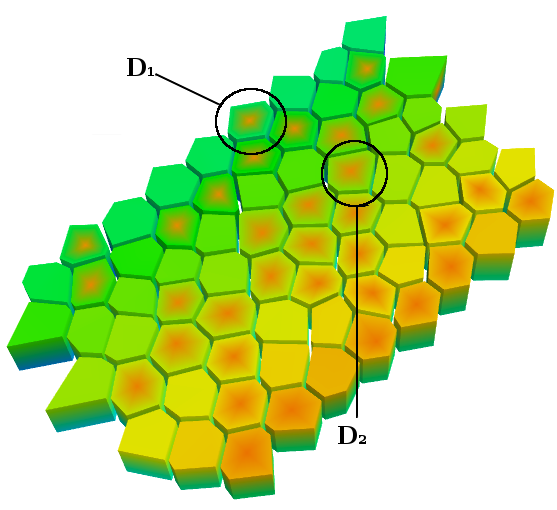
\includegraphics[width=3cm]{grains2.png} \vspace{1mm}
			
			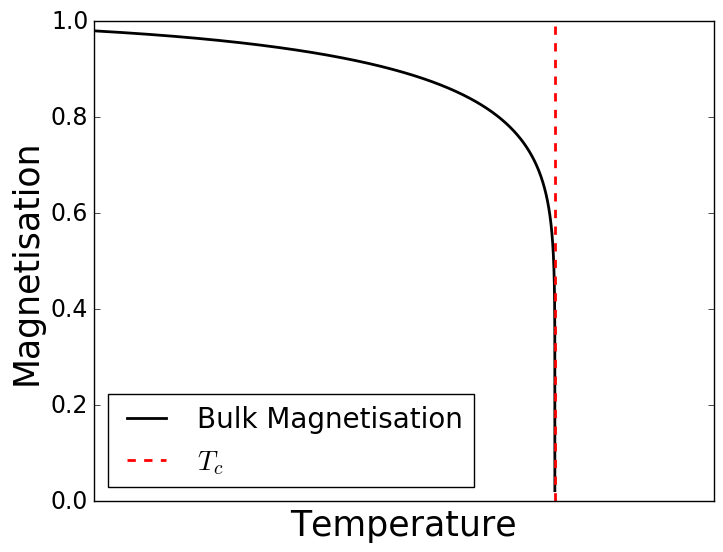
\includegraphics[width=4cm]{bulk.png}
		\end{center}
	\end{columns}
\end{frame}

\begin{frame}
	\frametitle{My Research}
	\begin{columns}
		\column{6cm}
		\begin{itemize}
			\item{Multiscale: The model is currently based upon three different scales}\newline
			\begin{enumerate}
				\item{Atomic Scale: Using \textbf{density functional theory} (DFT) techniques, the bonding between the atoms is modelled to find interaction strengths, lattice shape e.t.c.}\newline
				\item{Nano Scale: Using this information, the magnetic properties can be found for a grain at a number of temperatures}
			\end{enumerate}
		\end{itemize}
		\column{6cm}
		\begin{center}
			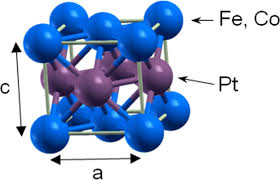
\includegraphics[width=4cm]{lattice.jpeg}\vspace{1mm}
			
			\tiny www.psi-k.org/newsletters/News{\_}89/Highlight{\_}89.pdf
		
			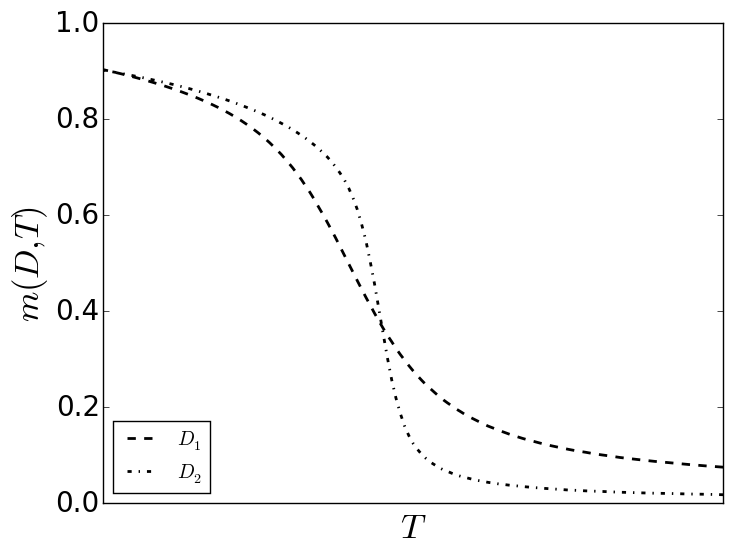
\includegraphics[width=4cm]{Ds_noinset.png}
		\end{center}
	\end{columns}
\end{frame}

\begin{frame}
	\frametitle{My Research}
	\begin{columns}
		\column{7cm}
		\begin{itemize}
			\item{Multiscale: The model is currently based upon three different scales}\newline
			\begin{enumerate}
				\setcounter{enumi}{2}
				\item{Macro Scale: With the magnetic properties of different sized grains, finite sized scaling (FSS) can be used to find the properties of any sized grain. \newline \newline From this point, the properties of the entire ensemble can be found with a distribution of grain sizes.}
			\end{enumerate}
		\end{itemize}
		\column{5cm}
		\begin{center}
			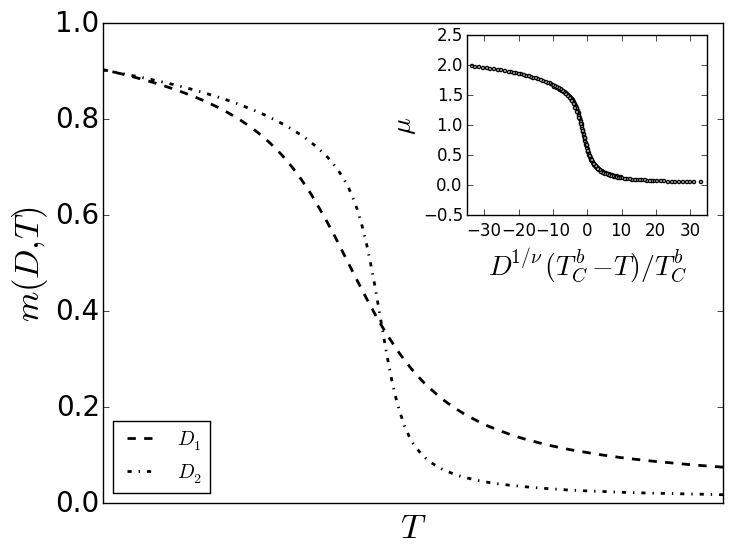
\includegraphics[width=4cm]{Ds.png} \\
			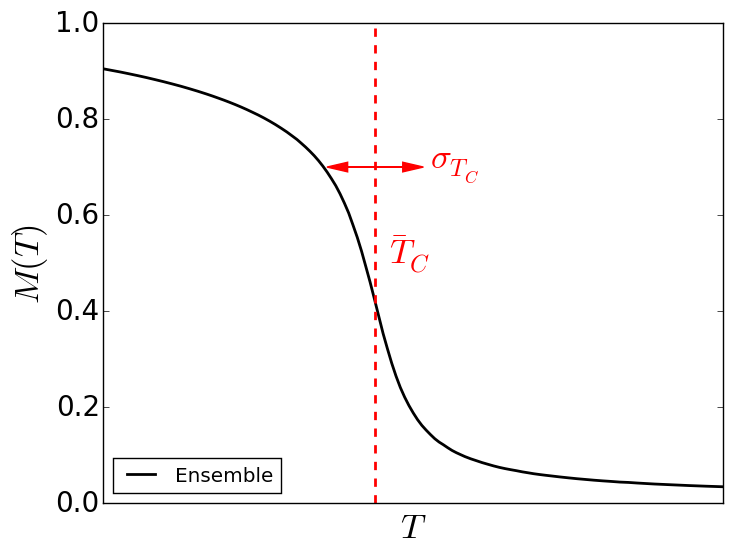
\includegraphics[width=4cm]{Aggregate.png}
		\end{center}
	\end{columns}
\end{frame}

\begin{frame}
	\frametitle{Applications}
	In Heat Assisted Magnetic Recording(HAMR)\footnotemark[1]:
	\begin{itemize}
		\item{Grains of the hard disk are heated to make them more easilly written}
		\item{$T_C$ distribution affects the noise performance}
		\item{Required for an areal density of up to 4Tb/in$^2$}
	\end{itemize} \vspace{5mm}
		
	\begin{center}
	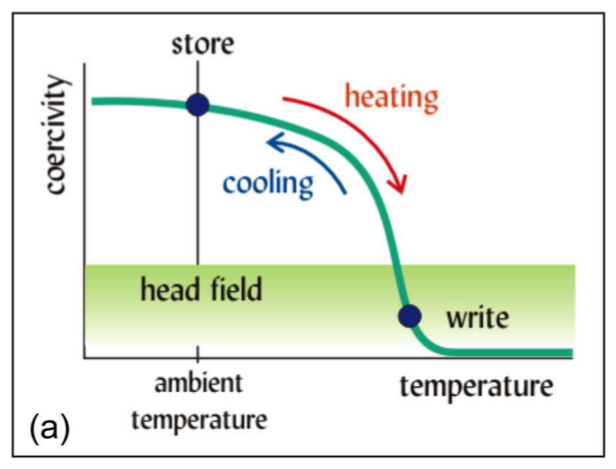
\includegraphics[width=4.5cm]{coerc.png} \hspace{2mm}
	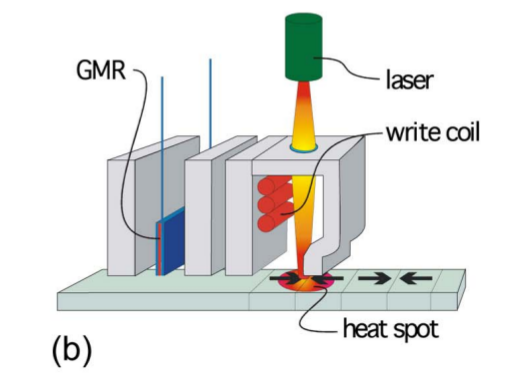
\includegraphics[width=4.5cm]{laser.png} \\
	\tiny E. Dobisz et al. Proc IEEE 96.11, 1836 (2008)
	\end{center}
	\footnotetext[1]{\tiny D. Weller et al. IEEE Transactions on Magnetics 50.1, 3100108 (2014)}
\end{frame}

\begin{frame}
	\frametitle{Applications}
	In Magnetic Hyperthermia Treatments\footnotemark[2]:
	\begin{itemize}
	\item{Magnetic nano-particles bind to the tumour cells}
	\item{They are heated using an alternating magnetic field}
	\item{Heating stops at $T_C$ allowing us to control the amount of tissue damage using grain sizes}
	\end{itemize}
		
	\begin{center}
	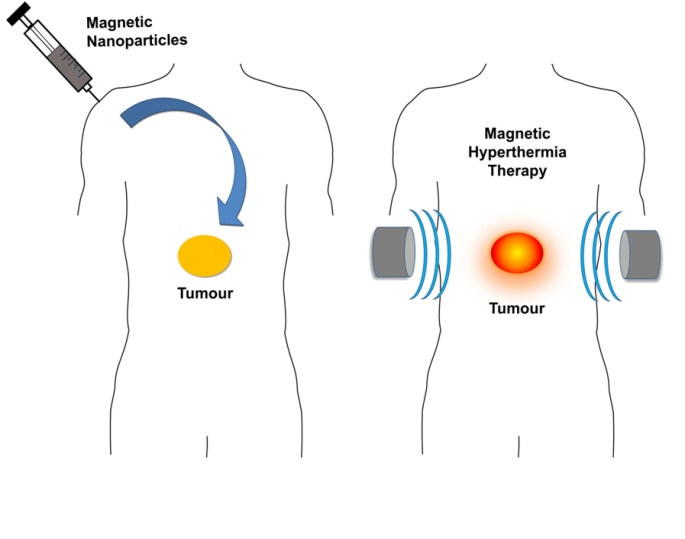
\includegraphics[width=4.5cm]{person.jpeg} \\
	\tiny \^{A}ngela Andrade et al. Coating Nanomagnetic Particles for Biomedical Applications (2011)
	\end{center}
	\footnotetext[2]{\tiny I Apostolova et al. Solid State Communications 149.25, 986 (2009)}
\end{frame}

\begin{frame}
	\frametitle{CDT in NGCM}
	\begin{columns}
		\column{7cm}
		The CDT has helped support this project through extensive training: \vspace{2mm}
		\begin{itemize}
			\item{Learnt 4 new programming languages}
			\begin{itemize}
				\item{Python, R, Julia, C}\vspace{2mm}
			\end{itemize}
			\item{Training in High Performance Computing (HPC)}
			\begin{itemize}
				\item{OpenMP, MPI, Intel Xeon Phi, GPU programming}\vspace{2mm}
			\end{itemize}
			\item{Software development skills}
			\begin{itemize}
				\item{Version control, virtual machines, continuous integration}\vspace{2mm}
			\end{itemize}
			\item{Numerical methods, Statistics.....}
		\end{itemize}
		\column{5cm}
		\begin{center}
			
\includegraphics[height=1.25cm]{julia.png}\\
			
\includegraphics[height=1cm]{python.png}
			
\includegraphics[height=1cm]{R.png} \vspace{14mm}
			
\includegraphics[height=1.5cm]{intel.jpg}\hspace{0.2cm}
			
\includegraphics[height=1.5cm]{nividia.png}
		\end{center}
	\end{columns}
\end{frame}

\begin{frame}
	\frametitle{CDT in NGCM}
	\begin{columns}
		\column{5cm}
		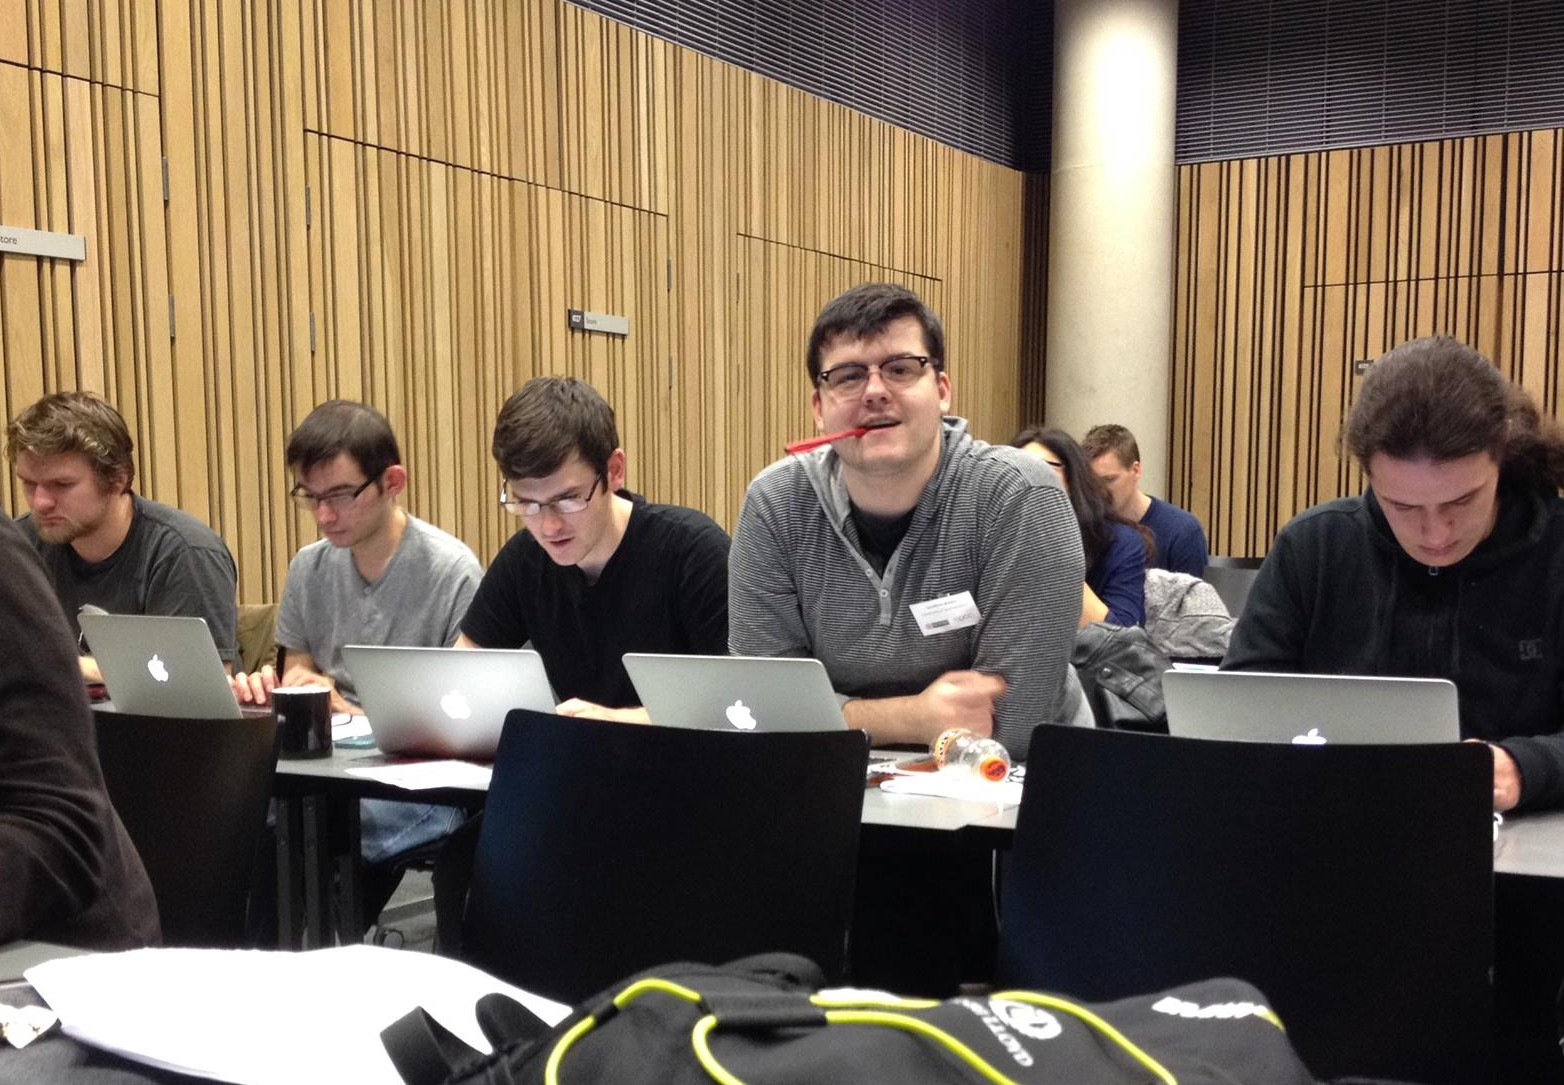
\includegraphics[width=5cm]{ngcm.jpg}
		\column{7cm}
		Freedom to explore my own interests through: \newline
		\begin{itemize}
			\item{Delivering a workshop on the Julia language}\newline
			\item{Individual research projects during the first year and summer}\newline
			\item{Organising and attending the NGCM Summer Academy}
		\end{itemize}
	\end{columns}
\end{frame}

\begin{frame}
	\begin{center}
		\huge{Thank you for listening}\vspace{2mm}
		
		\large{Contact: J.M.Waters@soton.ac.uk}
		
		\begin{itemize}
			\item{The CDT offers a number of courses year round: MPI, OpenMP, industry and technical seminars \newline ngcm.soton.ac.uk/ngcm-events}
			\item{The Summer Academy takes place in June \newline ngcm.soton.ac.uk/summer-academy}
			\item{\textbf{Today} at \textbf{4pm}: The CDT is running two training courses! }
			\begin{itemize}
				\item{Beginner Python Programming: Nuffield Theatre Room 1081 (6/1081) \newline cmg.soton.ac.uk/events/event-900}
				\item{Object Orientation in Python: Nuffield Theatre Room 1083 (6/1083) \newline cmg.soton.ac.uk/events/event-901}
			\end{itemize}
		\end{itemize}
	\end{center}
\end{frame}

\end{document}